\documentclass{standalone}
\usepackage{tikz}
\usetikzlibrary{patterns, positioning}


\begin{document}
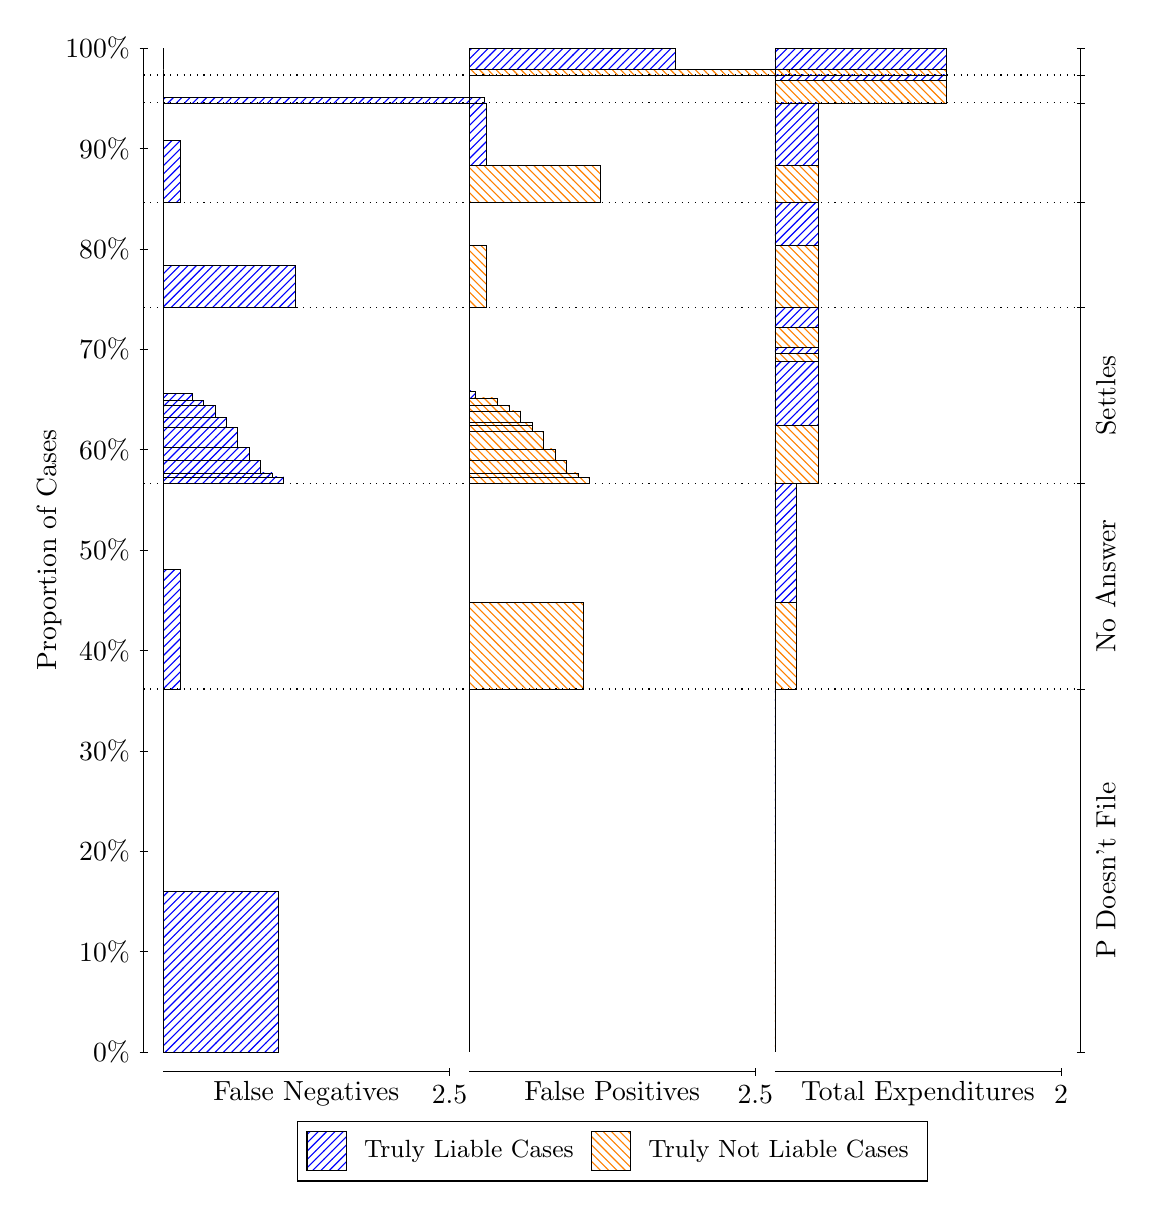
\begin{tikzpicture}
\draw[black, very thin] (1.5,1.75) -- (1.5,14.5);
\node[rotate=90, text=black, anchor=center] at (0.3, 8.125) {Proportion of Cases};
\draw[black, very thin] (1.45,1.75) -- (1.55,1.75);
\node[text=black, anchor=east] at (1.45, 1.75) {0\%};
\draw[black, very thin] (1.45,3.025) -- (1.55,3.025);
\node[text=black, anchor=east] at (1.45, 3.025) {10\%};
\draw[black, very thin] (1.45,4.3) -- (1.55,4.3);
\node[text=black, anchor=east] at (1.45, 4.3) {20\%};
\draw[black, very thin] (1.45,5.575) -- (1.55,5.575);
\node[text=black, anchor=east] at (1.45, 5.575) {30\%};
\draw[black, very thin] (1.45,6.85) -- (1.55,6.85);
\node[text=black, anchor=east] at (1.45, 6.85) {40\%};
\draw[black, very thin] (1.45,8.125) -- (1.55,8.125);
\node[text=black, anchor=east] at (1.45, 8.125) {50\%};
\draw[black, very thin] (1.45,9.4) -- (1.55,9.4);
\node[text=black, anchor=east] at (1.45, 9.4) {60\%};
\draw[black, very thin] (1.45,10.675) -- (1.55,10.675);
\node[text=black, anchor=east] at (1.45, 10.675) {70\%};
\draw[black, very thin] (1.45,11.95) -- (1.55,11.95);
\node[text=black, anchor=east] at (1.45, 11.95) {80\%};
\draw[black, very thin] (1.45,13.225) -- (1.55,13.225);
\node[text=black, anchor=east] at (1.45, 13.225) {90\%};
\draw[black, very thin] (1.45,14.5) -- (1.55,14.5);
\node[text=black, anchor=east] at (1.45, 14.5) {100\%};

\draw[black, very thin] (13.4,1.75) -- (13.4,14.5);
\draw[black, very thin] (13.35,1.75) -- (13.45,1.75);
\node[anchor=west] at (13.35, 1.75) {};
\draw[black, very thin] (13.35,6.3591) -- (13.45,6.3591);
\node[anchor=west] at (13.35, 6.3591) {};
\draw[black, very thin] (13.35,8.9729) -- (13.45,8.9729);
\node[anchor=west] at (13.35, 8.9729) {};
\draw[black, very thin] (13.35,11.202) -- (13.45,11.202);
\node[anchor=west] at (13.35, 11.202) {};
\draw[black, very thin] (13.35,12.535) -- (13.45,12.535);
\node[anchor=west] at (13.35, 12.535) {};
\draw[black, very thin] (13.35,13.803) -- (13.45,13.803);
\node[anchor=west] at (13.35, 13.803) {};
\draw[black, very thin] (13.35,14.158) -- (13.45,14.158);
\node[anchor=west] at (13.35, 14.158) {};
\draw[black, very thin] (13.35,14.5) -- (13.45,14.5);
\node[anchor=west] at (13.35, 14.5) {};

\draw[black, very thin, pattern color=blue, pattern=north east lines] (1.75,1.75) rectangle (3.2033,3.7943);
\draw[black, very thin, pattern color=orange, pattern=north west lines] (1.75,3.7943) rectangle (1.75,6.3591);
\draw[black, very thin, pattern color=blue, pattern=north east lines] (1.75,6.3591) rectangle (1.968,7.8751);
\draw[black, very thin, pattern color=orange, pattern=north west lines] (1.75,7.8751) rectangle (1.75,8.9729);
\draw[black, very thin, pattern color=blue, pattern=north east lines] (1.75,8.9729) rectangle (3.276,9.0542);
\draw[black, very thin, pattern color=blue, pattern=north east lines] (1.75,9.0542) rectangle (3.1307,9.1053);
\draw[black, very thin, pattern color=blue, pattern=north east lines] (1.75,9.1053) rectangle (2.9853,9.2647);
\draw[black, very thin, pattern color=blue, pattern=north east lines] (1.75,9.2647) rectangle (2.84,9.426);
\draw[black, very thin, pattern color=blue, pattern=north east lines] (1.75,9.426) rectangle (2.6947,9.6792);
\draw[black, very thin, pattern color=blue, pattern=north east lines] (1.75,9.6792) rectangle (2.5493,9.8088);
\draw[black, very thin, pattern color=blue, pattern=north east lines] (1.75,9.8088) rectangle (2.404,9.9583);
\draw[black, very thin, pattern color=blue, pattern=north east lines] (1.75,9.9583) rectangle (2.2587,10.028);
\draw[black, very thin, pattern color=blue, pattern=north east lines] (1.75,10.028) rectangle (2.1133,10.118);
\draw[black, very thin, pattern color=orange, pattern=north west lines] (1.75,10.118) rectangle (1.75,11.202);
\draw[black, very thin, pattern color=blue, pattern=north east lines] (1.75,11.202) rectangle (3.4213,11.74);
\draw[black, very thin, pattern color=orange, pattern=north west lines] (1.75,11.74) rectangle (1.75,12.535);
\draw[black, very thin, pattern color=blue, pattern=north east lines] (1.75,12.535) rectangle (1.968,13.325);
\draw[black, very thin, pattern color=orange, pattern=north west lines] (1.75,13.325) rectangle (1.75,13.803);
\draw[black, very thin, pattern color=blue, pattern=north east lines] (1.75,13.803) rectangle (5.8193,13.87);
\draw[black, very thin, pattern color=orange, pattern=north west lines] (1.75,13.87) rectangle (1.75,14.158);
\draw[black, very thin, pattern color=orange, pattern=north west lines] (1.75,14.158) rectangle (1.75,14.225);
\draw[black, very thin, pattern color=blue, pattern=north east lines] (1.75,14.225) rectangle (1.75,14.5);
\draw[black, very thin, pattern color=orange, pattern=north west lines] (5.6333,1.75) rectangle (5.6333,4.3148);
\draw[black, very thin, pattern color=blue, pattern=north east lines] (5.6333,4.3148) rectangle (5.6333,6.3591);
\draw[black, very thin, pattern color=orange, pattern=north west lines] (5.6333,6.3591) rectangle (7.0867,7.4569);
\draw[black, very thin, pattern color=blue, pattern=north east lines] (5.6333,7.4569) rectangle (5.6333,8.9729);
\draw[black, very thin, pattern color=orange, pattern=north west lines] (5.6333,8.9729) rectangle (7.1593,9.0485);
\draw[black, very thin, pattern color=orange, pattern=north west lines] (5.6333,9.0485) rectangle (7.014,9.1038);
\draw[black, very thin, pattern color=orange, pattern=north west lines] (5.6333,9.1038) rectangle (6.8687,9.2593);
\draw[black, very thin, pattern color=orange, pattern=north west lines] (5.6333,9.2593) rectangle (6.7233,9.4089);
\draw[black, very thin, pattern color=orange, pattern=north west lines] (5.6333,9.4089) rectangle (6.578,9.6314);
\draw[black, very thin, pattern color=orange, pattern=north west lines] (5.6333,9.6314) rectangle (6.4327,9.7066);
\draw[black, very thin, pattern color=orange, pattern=north west lines] (5.6333,9.7066) rectangle (6.4327,9.749);
\draw[black, very thin, pattern color=orange, pattern=north west lines] (5.6333,9.749) rectangle (6.2873,9.893);
\draw[black, very thin, pattern color=orange, pattern=north west lines] (5.6333,9.893) rectangle (6.142,9.961);
\draw[black, very thin, pattern color=orange, pattern=north west lines] (5.6333,9.961) rectangle (5.9967,10.057);
\draw[black, very thin, pattern color=blue, pattern=north east lines] (5.6333,10.057) rectangle (5.706,10.147);
\draw[black, very thin, pattern color=blue, pattern=north east lines] (5.6333,10.147) rectangle (5.6333,11.202);
\draw[black, very thin, pattern color=orange, pattern=north west lines] (5.6333,11.202) rectangle (5.8513,11.997);
\draw[black, very thin, pattern color=blue, pattern=north east lines] (5.6333,11.997) rectangle (5.6333,12.535);
\draw[black, very thin, pattern color=orange, pattern=north west lines] (5.6333,12.535) rectangle (7.3047,13.014);
\draw[black, very thin, pattern color=blue, pattern=north east lines] (5.6333,13.014) rectangle (5.8513,13.803);
\draw[black, very thin, pattern color=orange, pattern=north west lines] (5.6333,13.803) rectangle (5.6333,14.092);
\draw[black, very thin, pattern color=blue, pattern=north east lines] (5.6333,14.092) rectangle (5.6333,14.158);
\draw[black, very thin, pattern color=orange, pattern=north west lines] (5.6333,14.158) rectangle (9.7027,14.225);
\draw[black, very thin, pattern color=blue, pattern=north east lines] (5.6333,14.225) rectangle (8.2493,14.5);
\draw[black, very thin, pattern color=orange, pattern=north west lines] (9.5167,1.75) rectangle (9.5167,4.3148);
\draw[black, very thin, pattern color=blue, pattern=north east lines] (9.5167,4.3148) rectangle (9.5167,6.3591);
\draw[black, very thin, pattern color=orange, pattern=north west lines] (9.5167,6.3591) rectangle (9.7892,7.4569);
\draw[black, very thin, pattern color=blue, pattern=north east lines] (9.5167,7.4569) rectangle (9.7892,8.9729);
\draw[black, very thin, pattern color=orange, pattern=north west lines] (9.5167,8.9729) rectangle (10.062,9.7066);
\draw[black, very thin, pattern color=blue, pattern=north east lines] (9.5167,9.7066) rectangle (10.062,10.523);
\draw[black, very thin, pattern color=orange, pattern=north west lines] (9.5167,10.523) rectangle (10.062,10.619);
\draw[black, very thin, pattern color=blue, pattern=north east lines] (9.5167,10.619) rectangle (10.062,10.7);
\draw[black, very thin, pattern color=orange, pattern=north west lines] (9.5167,10.7) rectangle (10.062,10.955);
\draw[black, very thin, pattern color=blue, pattern=north east lines] (9.5167,10.955) rectangle (10.062,11.202);
\draw[black, very thin, pattern color=orange, pattern=north west lines] (9.5167,11.202) rectangle (10.062,11.997);
\draw[black, very thin, pattern color=blue, pattern=north east lines] (9.5167,11.997) rectangle (10.062,12.535);
\draw[black, very thin, pattern color=orange, pattern=north west lines] (9.5167,12.535) rectangle (10.062,13.014);
\draw[black, very thin, pattern color=blue, pattern=north east lines] (9.5167,13.014) rectangle (10.062,13.803);
\draw[black, very thin, pattern color=orange, pattern=north west lines] (9.5167,13.803) rectangle (11.697,14.092);
\draw[black, very thin, pattern color=blue, pattern=north east lines] (9.5167,14.092) rectangle (11.697,14.158);
\draw[black, very thin, pattern color=orange, pattern=north west lines] (9.5167,14.158) rectangle (11.697,14.225);
\draw[black, very thin, pattern color=blue, pattern=north east lines] (9.5167,14.225) rectangle (11.697,14.5);
\draw[black, dotted] (1.5,6.3591) -- (13.4,6.3591);
\draw[black, dotted] (1.5,8.9729) -- (13.4,8.9729);
\draw[black, dotted] (1.5,11.202) -- (13.4,11.202);
\draw[black, dotted] (1.5,12.535) -- (13.4,12.535);
\draw[black, dotted] (1.5,13.803) -- (13.4,13.803);
\draw[black, dotted] (1.5,14.158) -- (13.4,14.158);
\draw[black, very thin] (1.75,1.5) -- (5.3833,1.5);
\node[text=black, anchor=north] at (3.5667, 1.5) {False Negatives};
\draw[black, very thin] (5.3833,1.45) -- (5.3833,1.55);
\node[text=black, anchor=north] at (5.3833, 1.45) {2.5};

\draw[black, very thin] (5.6333,1.5) -- (9.2667,1.5);
\node[text=black, anchor=north] at (7.45, 1.5) {False Positives};
\draw[black, very thin] (9.2667,1.45) -- (9.2667,1.55);
\node[text=black, anchor=north] at (9.2667, 1.45) {2.5};

\draw[black, very thin] (9.5167,1.5) -- (13.15,1.5);
\node[text=black, anchor=north] at (11.333, 1.5) {Total Expenditures};
\draw[black, very thin] (13.15,1.45) -- (13.15,1.55);
\node[text=black, anchor=north] at (13.15, 1.45) {2};

\node[text=black, centered, rotate=90] at (13.72, 4.0546) {P Doesn't File};
\node[text=black, centered, rotate=90] at (13.72, 7.666) {No Answer};
\node[text=black, centered, rotate=90] at (13.72, 10.087) {Settles};





\draw (7.449999999999999,1.5) node[draw=none] (baseCoordinate) {};
\begin{scope}[align=center]
        \matrix[scale=0.5, draw=black, below=0.5cm of baseCoordinate, nodes={draw}, column sep=0.1cm]{
            \node[rectangle, draw, minimum width=0.5cm, minimum height=0.5cm, pattern color=blue, pattern=north east lines] {}; &
            \node[draw=none, font=\small, text=black] (B) {Truly Liable Cases}; &
            \node[rectangle, draw, minimum width=0.5cm, minimum height=0.5cm, pattern color=orange, pattern=north west lines] {}; &
            \node[draw=none, font=\small, text=black] (B) {Truly Not Liable Cases}; \\
            };
\end{scope}

\end{tikzpicture}
\end{document}